\section{Reingeniería de recurso no-ontológicos}
Debido a que se utilizó recursos no-ontológicos, debemos de realizar un proceso de reingeniería para transformar estos recursos de manera a incluir esa información en la ontología. Procedemos de esta manera al proceso de reingeniería del esquema de publicación de OCDS.


\subsection{Ingeniería reversa del recurso no-ontológico}
El primer paso es analizar el recurso no-ontológico para identificar los principales componentes y crear representaciones del recurso. Dentro de esta actividad procederemos a la recolección de los datos, la abstracción conceptual y exploración de la información.

\subsubsection{Recolección de datos}

El propósito de esta actividad es buscar y recolectar todos los datos y la documentación del recurso no-ontológico incluyendo su propósito, componentes, modelo de datos y detalles de implementación.

El OCDS es un estándar abierto de datos para la publicación de información estructurada sobre todas las etapas de un proceso de contratación: desde la planificación hasta la implementación.

La publicación de los datos siguiendo el OCDS permite una mayor transparencia en la contratación pública y puede apoyar al análisis accesible y a profundidad de la eficiencia, efectividad, equidad e integridad de los sistemas de contratación pública. El OCDS fue diseñado con un enfoque en la contratación pública de bienes, obras y servicios, pero puede ampliarse para su uso en otros contextos. 

El OCDS se centra en las siguientes necesidades del usuario:
\begin{itemize}
    \item Fortalecimiento de la transparencia, rendición de cuentas e integridad de los contratos públicos.
    \item Hacer un buen uso del dinero del gobierno.
    \item Permitir al sector privado una competencia justa por contratos públicos.
    \item Control de la eficacia de la prestación de servicios. 
\end{itemize}

El OCDS posee un sitio web donde se encuentra documentado todo el estándar, soportando los idiomas español, inglés y francés. Además posee una guía de implementación del estándar \footnote{http://standard.open-contracting.org/latest/en/implementation/}, un validador de la estructura sintáctica del mismo \footnote{http://standard.open-contracting.org/review/} y un mecanismo de gestión de extensiones \footnote{http://standard.open-contracting.org/latest/en/extensions/}.

\subsubsection{Modelo conceptual}

En esta actividad se identifica el esquema de recursos así como también los componentes conceptuales y sus relaciones. Además se crea un modelo conceptual dividido por bloques de conceptos relacionados. El conocimiento se expresa mediante representaciones primitivas de conceptos y relaciones entre conceptos. A continuación se representa la conceptualización teniendo como base el OCDS.

Un proceso de contratación se define como toda la información relativa a la planificación, la licitación, las adjudicaciones, los contratos y la ejecución de contratos relacionados con un solo proceso de iniciación.

Un proceso de contratación agrupa información sobre diferentes etapas o fases relacionadas a la vida útil de un contrato, a partir de la planificación, progresando a través de las etapas de iniciación u oferta, luego por la adjudicación y contrato y finalizando con la implementación del producto o servicio como se muestra en la Figura \ref{img:fases del proceso licitatorio }.

\begin{figure}[!htbp]
    \centering
    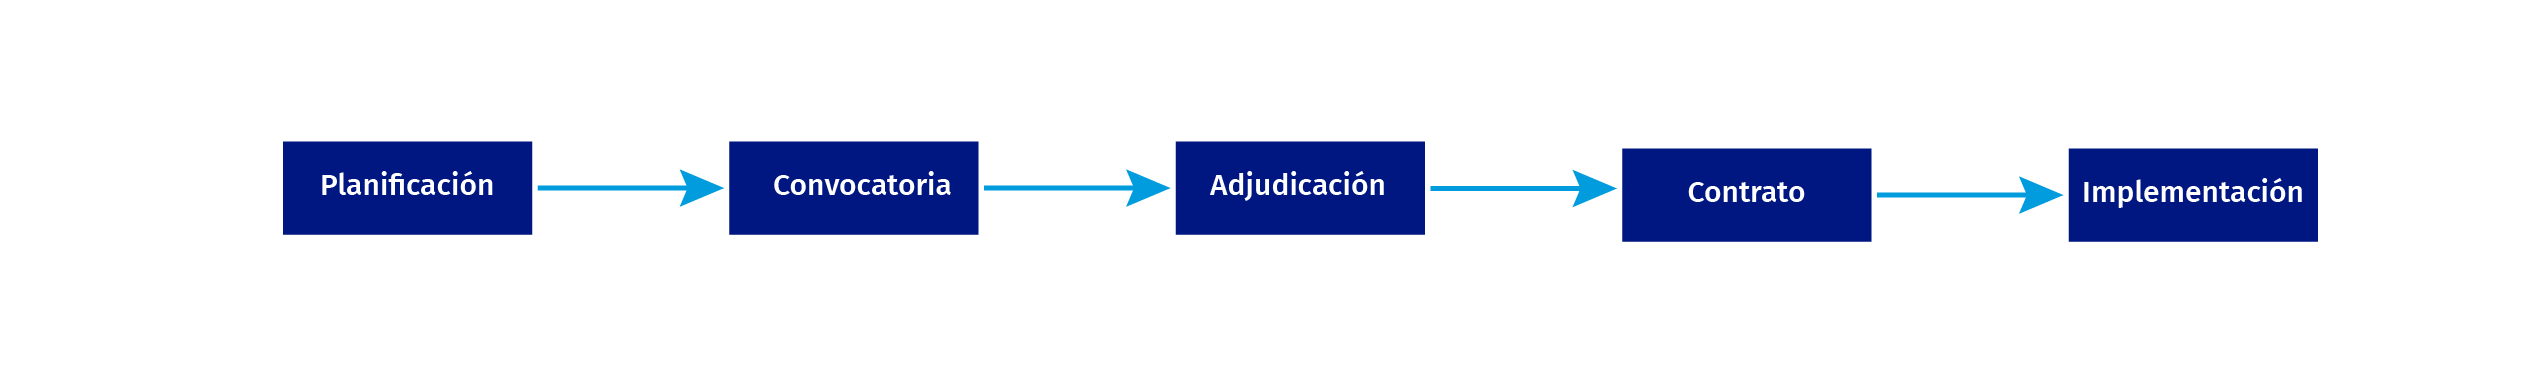
\includegraphics[width=150mm]{figuras/Diagramas_ProcesoLicitatorio.png}
    \caption{Modelo de fases del Proceso Licitatorio}
    \label{img:fases del proceso licitatorio }
\end{figure}

Las etapas son correlativas, esto significa que necesariamente debe de existir la etapa anterior antes de existir la siguiente. Todas las etapas representan un bloque de información.

Además de estas etapas existe otro concepto importante que es el bloque de Organización, que puede corresponder tanto al comprador como al oferente. Esta Organización puede estar ligada a cualquiera de las etapas del proceso de contratación. A continuación se detallan cada una de las etapas.
\paragraph{Planificación (\textit{Planning})}\hfill \break
Este bloque contiene información necesaria para describir los antecedentes de un proceso de contratación y puede incluir detalles del presupuesto del que se extraen los fondos o proyectos relacionados. Todo proceso de contratación posee una única planificación, dicha planificación tiene un presupuesto (budget) asociado donde finalmente se indica el valor o monto estimado para la adquisición del bien o servicio. Un diagrama de los componentes principales de la clase Planificación puede verse en la Figura \ref{img:Fase de Planificacion}.

\begin{figure}[htbp!]
    \centering
    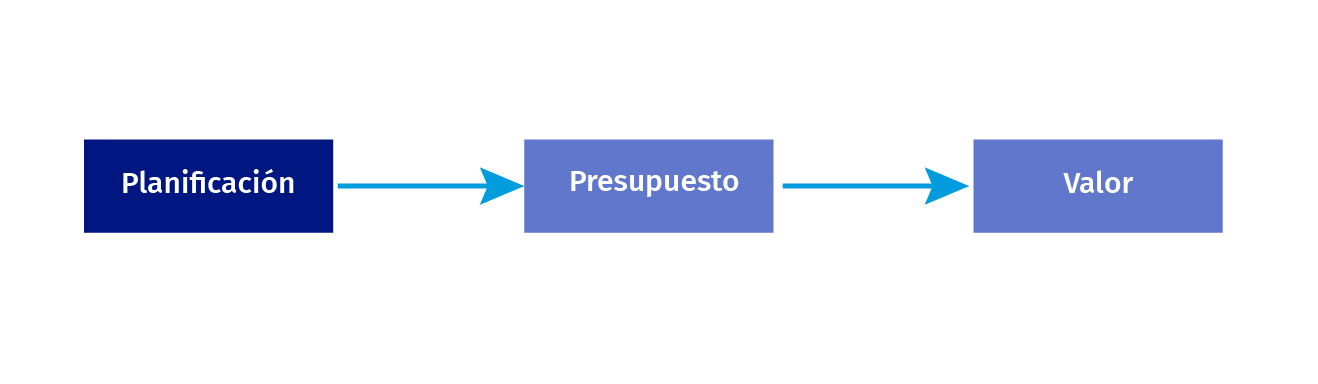
\includegraphics[width=150mm]{figuras/Diagramas_Planificacion.png}
    \caption{Modelo de fase de Planificación}
    \label{img:Fase de Planificacion}
\end{figure}

\paragraph{Convocatoria (\textit{Tender})}\hfill \break
Este bloque incluye detalles del anuncio indicando que una organización tiene la intención de abastecerse de algunos bienes o servicios y establecer uno o más contratos para estos. Todo proceso de contratación posee una única convocatoria, dicha convocatoria tiene asociada la organización involucrada en el proceso. Además, la convocatoria indica los ítems requeridos, el período establecido, los documentos utilizados, las adendas que pudieran haberse realizado sobre la convocatoria original y la lista de hitos. Se observa el esquema en la Figura \ref{img:Fase de Convocatoria}

\begin{figure}[htbp!]
    \centering
    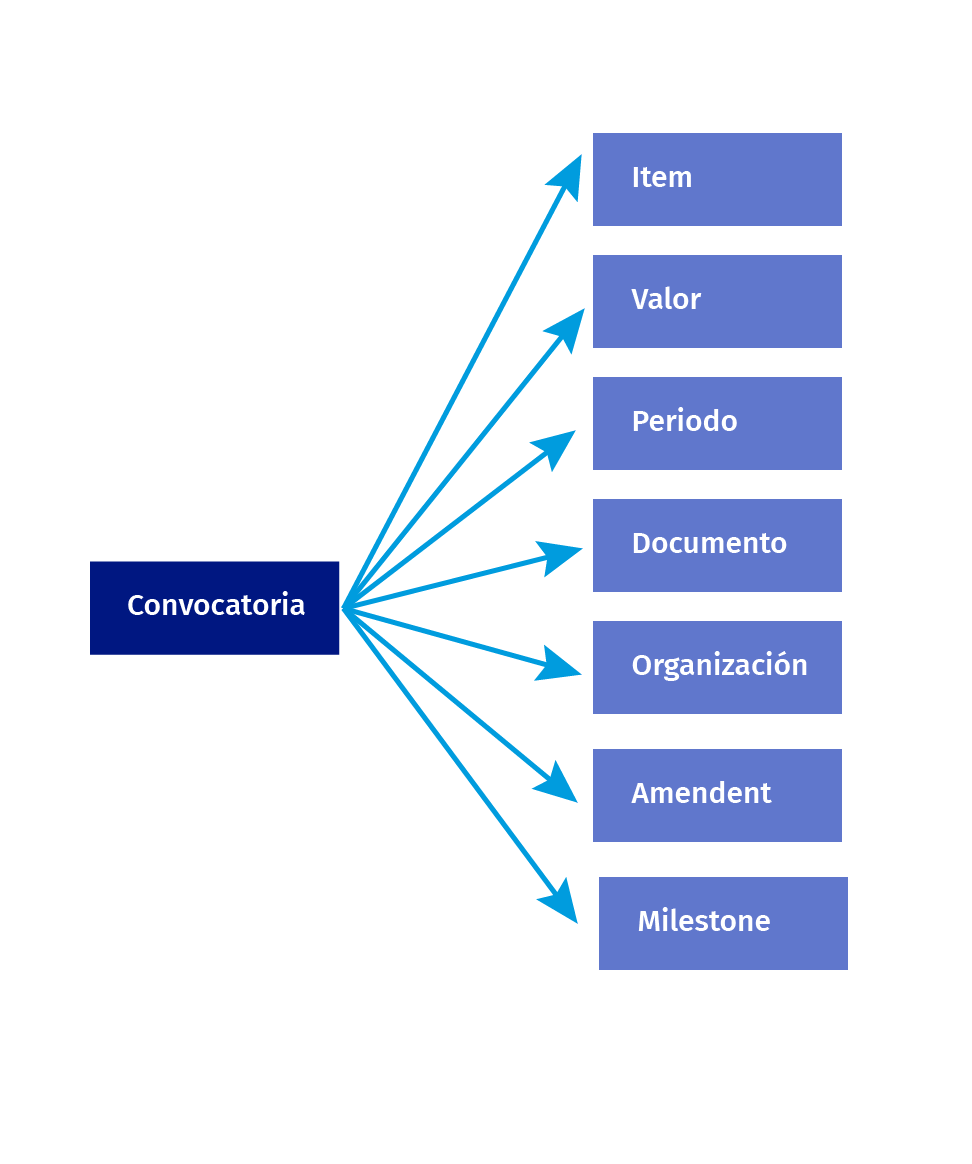
\includegraphics[width=150mm]{figuras/Diagramas_Convocatoria.png}
    \caption{Modelo de fase de Convocatoria}
    \label{img:Fase de Convocatoria}
\end{figure}

\paragraph{Adjudicación (\textit{Award})}\hfill \break
Este bloque se utiliza para anunciar las adjudicaciones emitidas para una licitación. Todo proceso de contratación puede involucrar una o más adjudicaciones, dichas adjudicaciones indican, para cada proveedor (organización), los ítems adjudicados, el valor o monto adjudicado y los documentos asociados al proceso. Esto se aprecia en la Figura \ref{img:Fase de Adjudiacion}


\begin{figure}[htbp!]
    \centering
    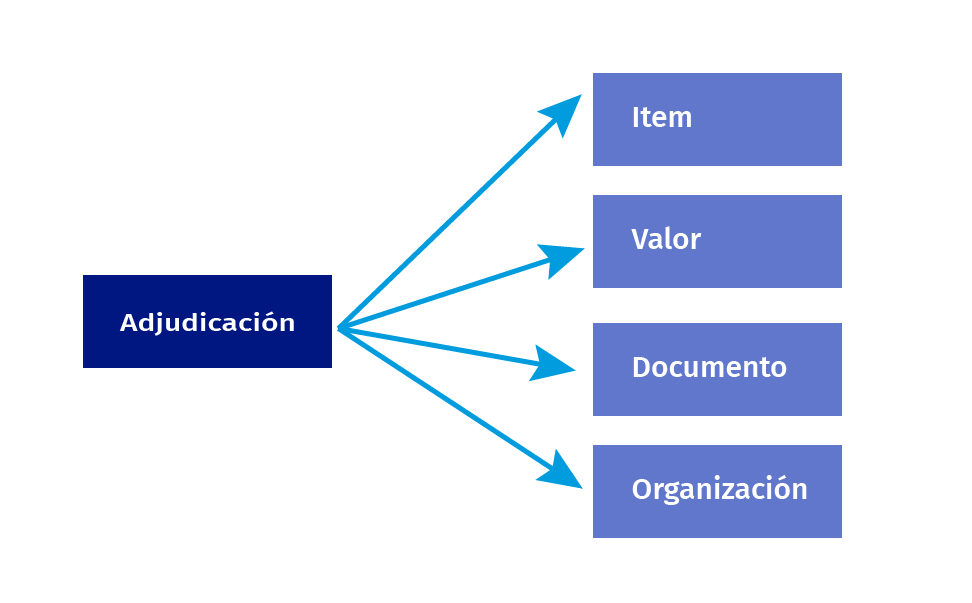
\includegraphics[width=150mm]{figuras/Diagramas_Adjudicacion.png}.
    \caption{Modelo de fase de Adjudicación}
    \label{img:Fase de Adjudiacion}
\end{figure}


\paragraph{Contrato (\textit{Contract})}\hfill \break
Este bloque se utiliza para proporcionar detalles de los contratos que se han celebrado. Todo proceso de contratación puede involucrar uno o más contratos, cada uno de los cuales debe estar asociado a una adjudicación específica. El proveedor (organización) adjudicado está indicado en la adjudicación, no así en el contrato. El contrato también indica los ítems adjudicados, los documentos asociados al proceso y la implementación del contrato. La implementación del contrato contiene información acerca de los hitos, las transacciones realizadas y los documentos utilizados. En la Figura \ref{img:Fase de Contrato} vemos un esquema de la estructura del Contrato.

\begin{figure}[htbp!]
    \centering
    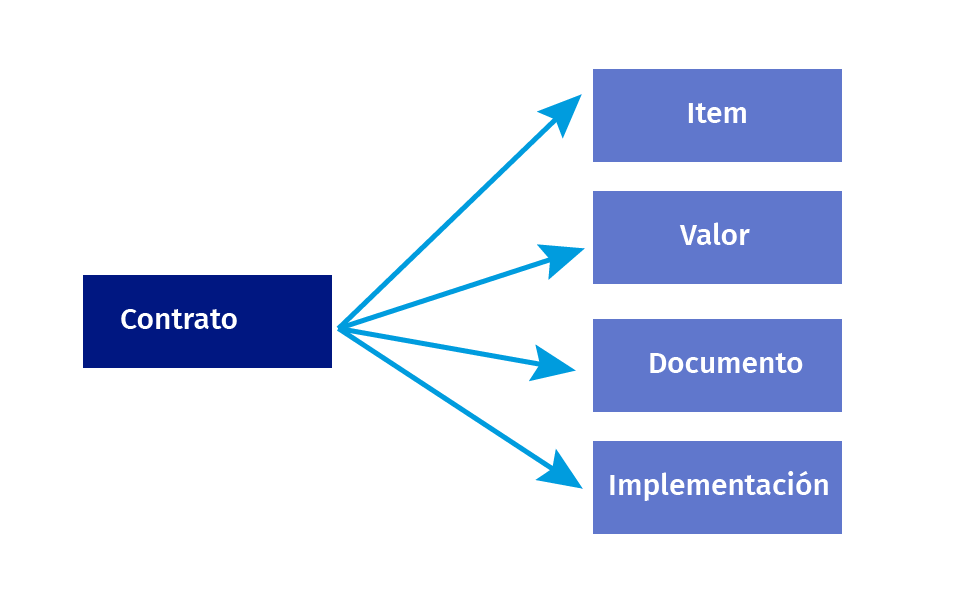
\includegraphics[width=150mm]{figuras/Diagramas_Contrato.png}
    \caption{Modelo de fase de Contrato}
    \label{img:Fase de Contrato}
\end{figure}

\paragraph{Otros componentes del estándar}\hfill \break
El estándar posee además otros componentes o bloques que agrupan y contienen metadatos de publicación de los datos.  A continuación se detallan dichos componentes.

\paragraph{\textit{Releases}}\hfill \break
Para fomentar la mayor apertura de información el estándar está preparado para publicar la información en tiempo real. En cada etapa del proceso de contratación o con cada cambio que ocurra sobre los datos, el estándar prevé la publicación de esa nueva porción de información mediante releases.
Los releases son acumulativos, es decir, durante un proceso de contratación se pueden proporcionar uno o más releases, por ejemplo: describir una licitación, anunciar la adjudicación de contratos y proporcionar actualizaciones sobre los mismos.
Una vez que un release ha sido publicado no puede cambiar. La información actualizada debe ser compartida a través de un nuevo release.
Los releases pueden ser publicados a través de un único sistema o de manera distribuida por diferentes sistemas, pero todos éstos deben estar relacionados a partir de un identificador único denominado Open Contracting ID (OCID).

\paragraph{\textit{Releases}}\hfill \break
Un registro (\textit{Record}) de contratación provee una instantánea del proceso de contratación en un punto dado en el tiempo, que reúne todas las versiones por las cuales pasó ese proceso en un solo lugar.
Un Record contiene tres elementos clave: 
\begin{itemize}
    \item Una lista de todos los releases asociados a un proceso de contratación en particular, 
    \item Un release compilado que contiene la última versión de los datos,
    \item Una versión histórica de releases que contiene la historia con todos los cambios realizados sobre los datos.
\end{itemize}

\paragraph{\textit{Release package}}\hfill \break
Un release package es un esquema de agrupación para la publicación de releases, describe el documento contenedor y metadatos para la publicación de releases.

\paragraph{\textit{Record package}}\hfill \break
Un Record Package es un esquema de agrupación para la publicación de Records, describe el documento contenedor y metadatos para la publicación de Records. En la Figura \ref{img:Record Package} se muestra el modelo conceptual de \textit{Record Package}.



\begin{figure}[ht!]
    \centering
    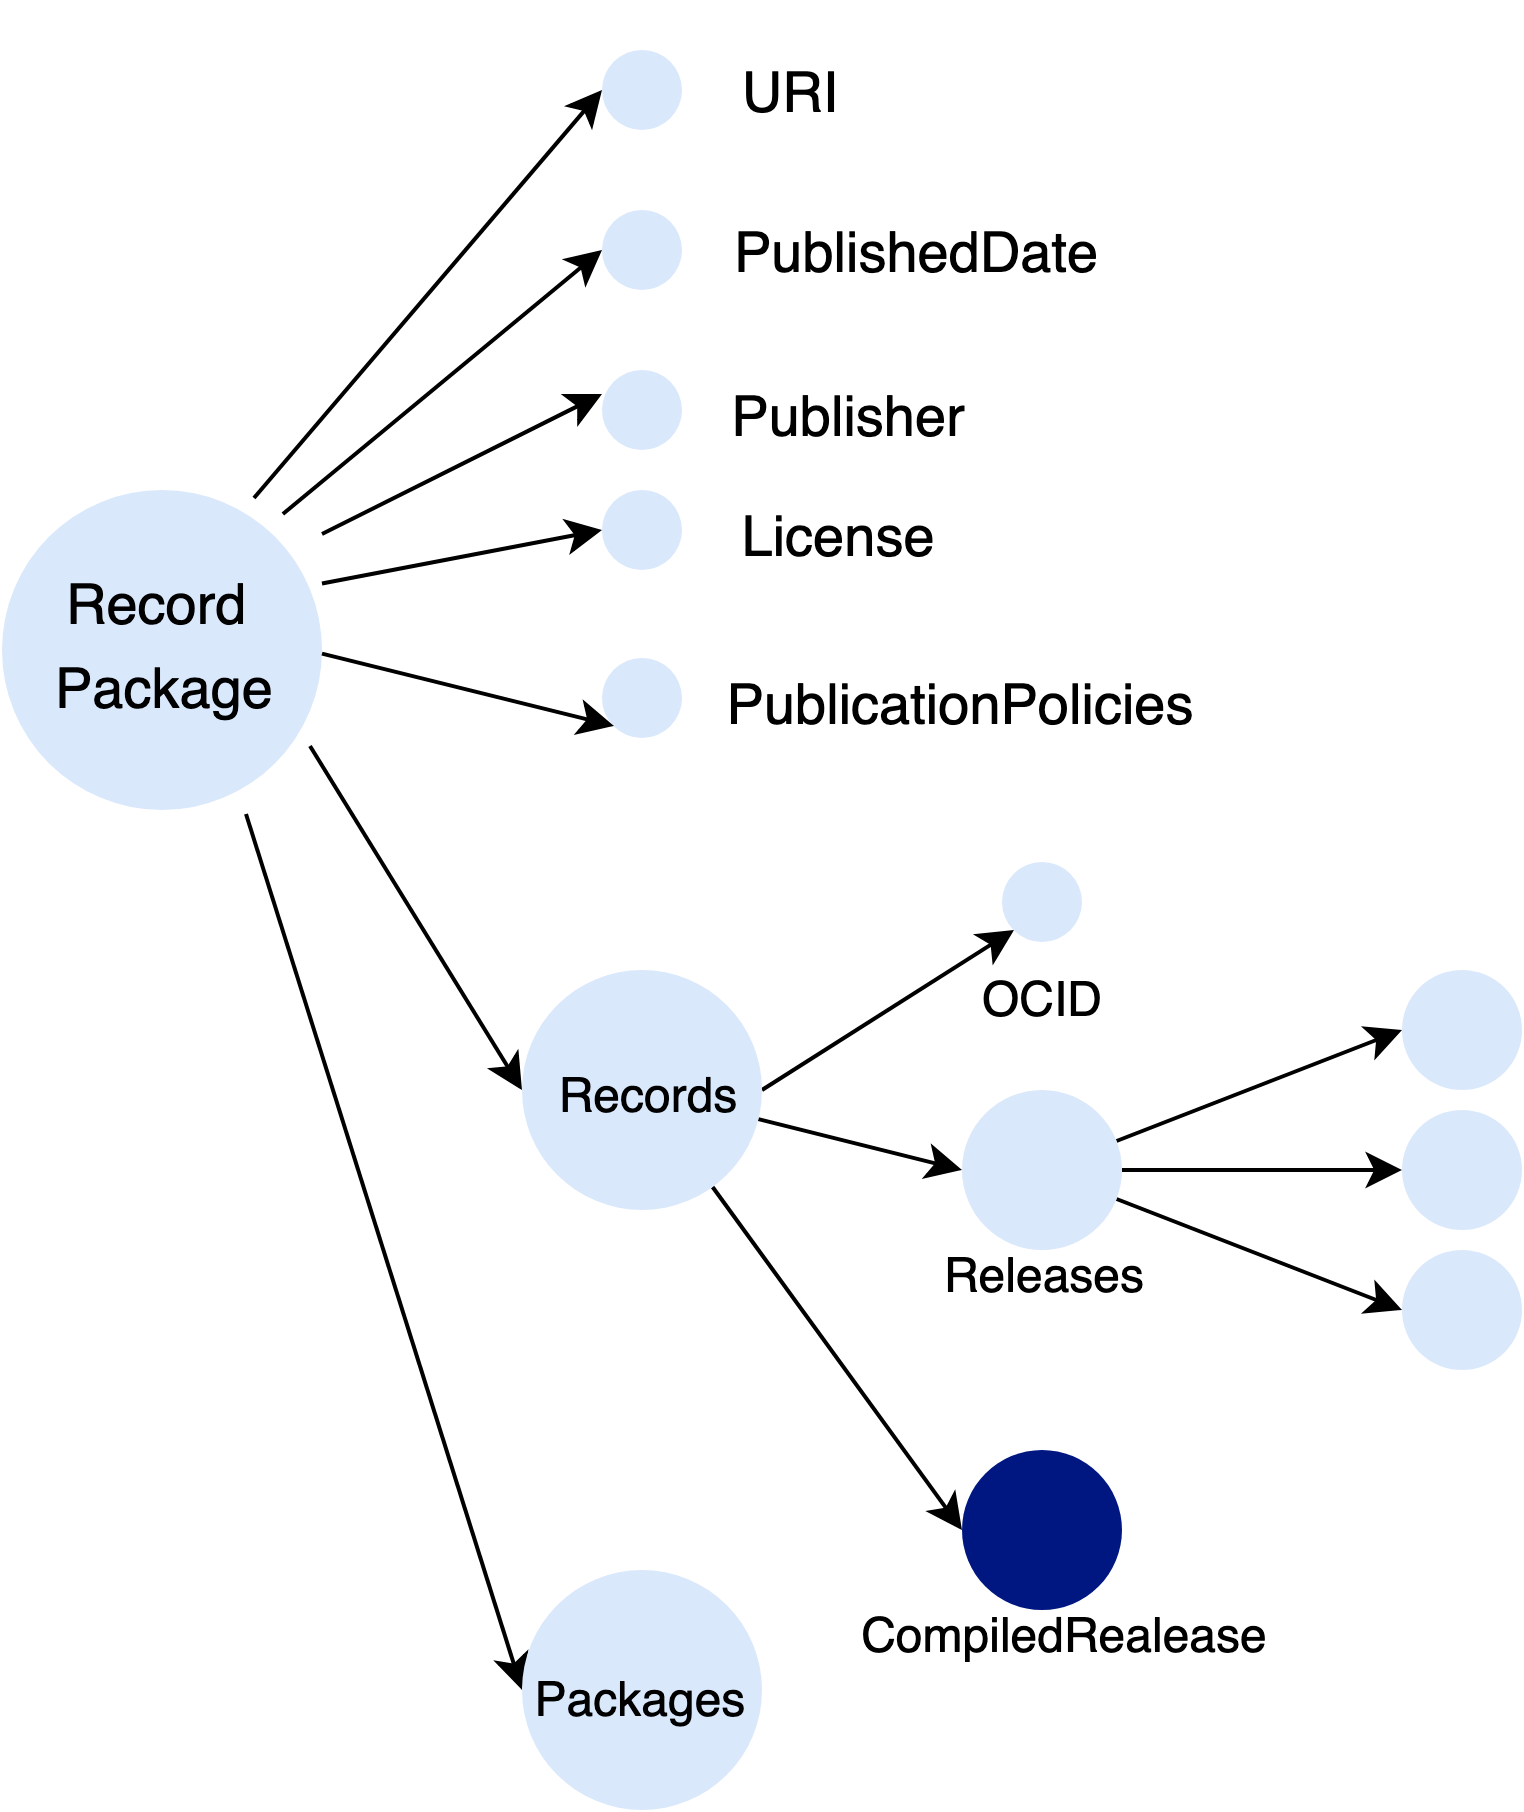
\includegraphics{figuras/Diagramas-RecordPackage.png}
    \caption{Record Package}
    \label{img:Record Package}
\end{figure}


\subsubsection{Transformación del recurso no-ontológico}
En esta sección se utilizaron los patrones de diseño para seguir construyendo un modelo conceptual y luego proseguir con la implementación de la ontología. 
\paragraph{Búsqueda de Patrones de Diseño}\hfill \break
El objetivo de este paso es buscar posibles patrones de diseño que conviertan el recurso no-ontológico en un modelo conceptual. 
Una vez analizado el esquema del OCDS se procedió a la búsqueda de patrones de diseño de ontologías, se utilizó el repositorio ontologydesingpatterns.org para realizar esta búsqueda de patrones bien conocidos por la comunidad de desarrolladores de ontologías y recomendado por la metodología NeOn.
Los patrones que son relevantes son aquellos que involucran tiempo, dinero, empresas u organizaciones, lugares y procesos en general. Luego de una búsqueda se encontraron los siguientes patrones de diseño que podrían ser útiles al momento del desarrollo de la ontología.
\begin{enumerate}
    \item Intervalo de tiempo\footnote{http://ontologydesignpatterns.org/wiki/Submissions:TimeInterval}
    \item Precio\footnote{http://ontologydesignpatterns.org/wiki/Submissions:Price} 
    \item Etiquetas\footnote{http://ontologydesignpatterns.org/wiki/Submissions:Tagging}
    \item Lugar\footnote{http://ontologydesignpatterns.org/wiki/Submissions:Place}
    \item Lista\footnote{http://ontologydesignpatterns.org/wiki/Submissions:List}
    \item Secuencia\footnote{http://ontologydesignpatterns.org/wiki/Submissions:Sequence}
    \item Boleta de Pago\footnote{http://ontologydesignpatterns.org/wiki/Submissions:Invoice} 
\end{enumerate}

Además se investigaron otros patrones de reingeniería, pero ninguno de éstos se adecuaba ya que están orientados a patrones jerárquicos de diseño y el dominio modela una secuencia o proceso. 

Se creó un patrón de conversión del estándar de documentacion JSON SCHEMA http://json-schema.org/ a un modelo ontológico. El patrón de conversión tiene los siguientes lineamientos.

\begin{itemize}
    \item Todos los objetos JSON del esquema son potenciales conceptos de la ontología desarrollada. Un Objeto JSON será considerado como clase o individuo en el modelo conceptual.
    \item El hecho de que un objeto esté relacionado a otro no necesariamente indica una relación de jerarquía, puede a la vez tratarse de una relación de contención, uso, correlación o dependencia.
    \item Todos los atributos de un Objeto JSON de tipo \textit{string} o numérico son potenciales propiedades (en la ontología) del concepto generado a partir el Objeto JSON.
    \item Los tipos de datos nos indican el tipo de dato en el formato RDF. Por ejemplo, si dentro de JSON Schema tenemos un campo que solo acepta números, podemos decir que esa propiedad es de tipo \textit{xsd:long}. Así, pueden ser una restricción en los valores de la propiedad.
    \item El nombre del objeto JSON es un candidato para nombrar esta relación. Por ejemplo, un presupuesto posee un objeto de nombre monto, de tipo valor. Por lo que podemos decir que el nombre de la relación entre presupuesto y valor se llamará monto.
    \item Los arreglos son representados a través de la relación uno a muchos dentro del modelo ontológico.
    \item Los atributos \textit{id}, \textit{identifier} o similares son potenciales identificadores de las instancias de cada concepto.
    
\end{itemize}

El esquema del OCDS posee una lista de códigos (\textit{Codelist}) de dos tipos, abiertos y cerrados. Los \textit{Codelist} Abiertos proveen códigos sugeridos, los publicadores pueden extender esta lista con nuevos códigos sin el consenso de otros publicadores. Mientras que los \textit{Codelist} Cerrados proveen códigos mandatorios, los publicadores solo pueden utilizar los valores de la lista oficial, cambios a \textit{Codelist} cerrados deben hacerse a través de la gobernanza y revisión de la lista. Esta lista de códigos fueron transformados utilizando el patrón mencionado a continuación. 

Para los \textit{Codelist} Abiertos se los convirtió en \textit{individuals}, en otros términos, instancias de los conceptos. Para los \textit{Codelist} Cerrados  se los convirtió en \textit{Enumerated Classes}. Las \textit{Enumerated Classes} impiden la declaración de nuevos individuos que pertenecen a esta clase, siendo así más restrictivos.
\paragraph{Utilización de patrones}\hfill \break
Por último, se consideraron los patrones mencionados anteriormente para los siguientes conceptos:
Para el concepto \textit{Value} del OCDS, que representan valores monetarios, se utilizó el patrón \textit{Price}. El patrón describe el precio de alguna entidad, dicho precio contiene un valor y una moneda. En la Figura \ref{img:Modelo de Precio} se muestra el diagrama del patrón.

\begin{figure}[ht!]
    \centering
    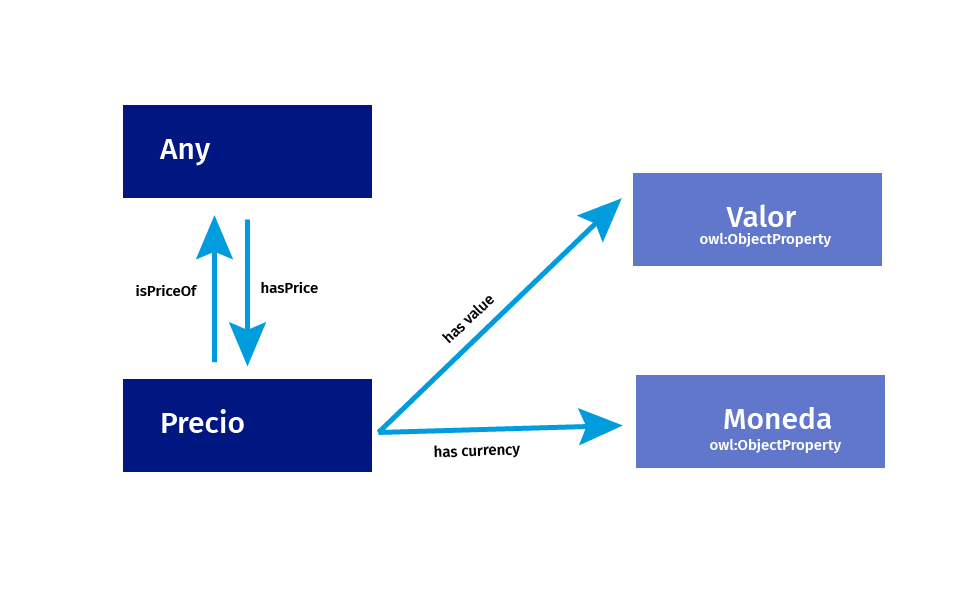
\includegraphics[width=150mm]{figuras/Diagramas_Precio.png}
    \caption{Modelo de Precio}
    \label{img:Modelo de Precio}
    
\end{figure}

En cuanto a la implementación, se optó por mantener \textit{Value} y \textit{Currency} como \textit{DataType properties} para mantener la simplicidad de nuestra ontología.

Para el concepto \textit{Period}, que representan periodos de tiempo se utilizó el patrón \textsc{Time Interval}. El patrón describe un intervalo de tiempo que contiene una fecha de inicio, una fecha de fin y una fecha del intervalo. Un posible uso del patrón sería la fecha “Agosto del 2018” tiene un fecha de inicio “1 de Agosto” y una fecha de fin “31 de Agosto”. En la implementación se omitió la propiedad Intervalo de tiempo, ya que no es necesaria para este este dominio. El modelo se puede ver en la Figura \ref{img:Modelo de Intervalo de precio}.

\begin{figure}[ht!]
    \centering
    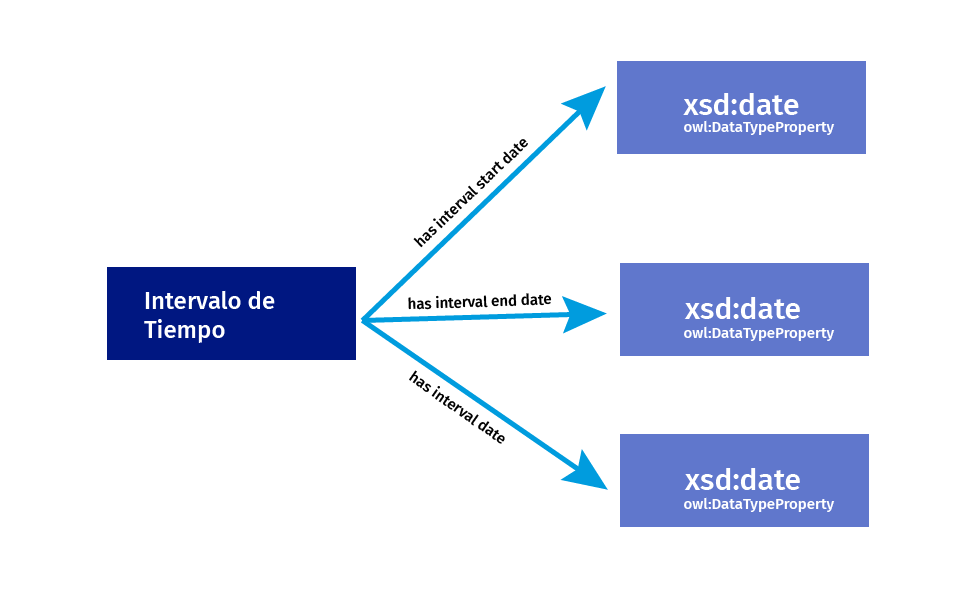
\includegraphics[width=150mm]{figuras/Diagramas_Tiempo.png}
    \caption{Modelo de Intervalo de tiempo}
    \label{img:Modelo de Intervalo de precio}
    
\end{figure}

Para la relación que existe entre \textit{Planning, Tender, Award, Contract e Implementation}, que tienen una relación de dependencia y de secuencia, se utilizó el patrón \textit{Sequence}. El patrón describe una secuencia de hecho a través de las propiedades Precede, Precede Directamente, Antecede y Antecede Directamente. Por ejemplo, decidir qué camisa utilizaré precede directamente a colocarse la camisa, y precede a colocarse la corbata. En la Figura \ref{img:Modelo de dependencia y secuencia} se presenta el diagrama del patrón. Se utilizó este patrón para describir la secuencia del proceso de contrataciones.

\begin{figure}[ht!]
    \centering
    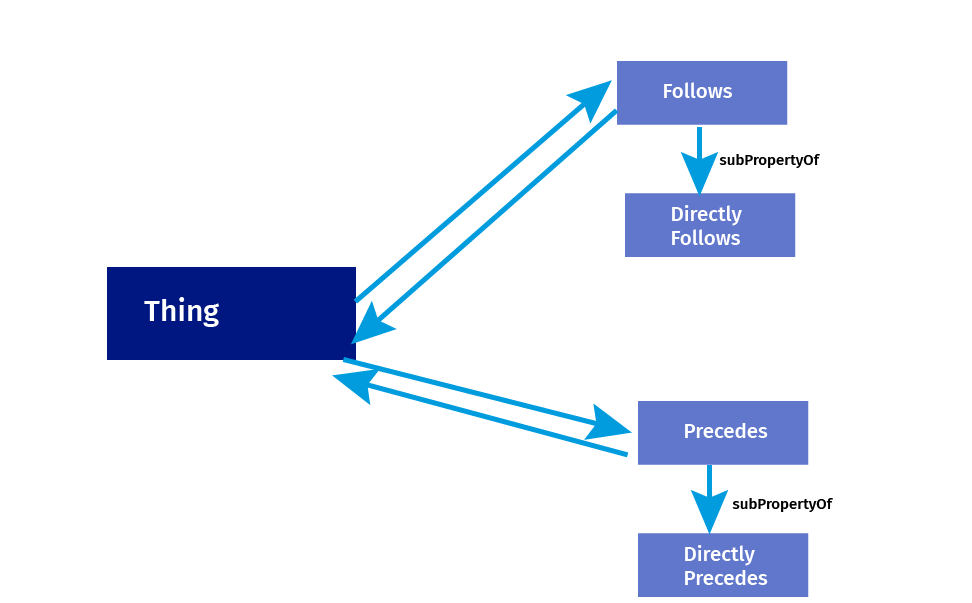
\includegraphics[width=150mm]{figuras/Diagramas_Follows.png}
    \caption{Modelo de dependencia y secuencia}
    \label{img:Modelo de dependencia y secuencia}
    
\end{figure}

\subsubsection{Construcción de la ontología}

Una vez concluido el modelo conceptual de la ontología procedemos a la construcción de la misma utilizando el lenguaje OWL y la herramienta Protégé.

Dentro de la fase de búsqueda de recursos Ontológicos, se encontró una ontología desarrolladas\footnote{https://github.com/ColinMaudry/open-contracting-ld} por un colaborador al proyecto OCD, la ontología siguió una transformación directa de JSON SCHEMA del estándar, la misma representa un punto de partida para seguir desarrollando la ontología. De esta manera además queremos incentivar la colaboración y hacer partícipe a toda la comunidad del OCDS.

El primer paso fue importar la ontología al software Protégé. Al hacer esto el software reestructuró el código de la ontología e hizo inferencias básicas detalladas a continuación. La estructura del documento del cual se partió estaba agrupada según conceptos semánticos relacionados. Protégé estructuró la ontología según sean \textit{Annotation Property, DataType Property u Object property} y luego ordenó de forma alfabética tomando como referencia el nombre de la propiedad.

Se encontraron algunas inconsistencias sintácticas dentro de la ontología, debido a que la misma fue hecha sin utilizar ninguna herramienta para desarrollo de ontologías, lo cual da lugar a errores sintácticos. Por ejemplo, el rango de la clase \textit{FormerValue} estaba definido como \textit{xsd:Integer}, Protégé infiere de que se trataba de un nuevo tipo de dato,  debido a que no existe este tipo de dato sino que debe ser \textit{xsd:integer}. Así también otro error en el documento en donde se escribió \textit{commnent} en lugar de \textit{commnent}, inmediatamente Protégé infiere como un nuevo tipo de dato. Como aprendizaje, el uso de una herramienta ontológica como Protégé nos ayuda a prevenir errores de sintaxis en la creación de la ontología y además acelera el proceso de desarrollo gracias a una interfaz gráfica que nos ayuda a distinguir entre Clases, \textit{DataType Properties} por citar algunas funcionalidades.

Toda la ontología inicial utilizó el tipo \textit{rdf:Property} para definir las propiedades. Debido a que \textit{owl:ObjectProperty} y \textit{owl:DataTypeProperty} son subclases de \textit{Property}, se decidió especializar las relaciones con estas subclases. Las propiedades que relacionan dos instancias fueron asignadas como owl:ObjectProperty y las propiedades relacionadas entre una instancia y un valor fueron asignadas como owl:DataTypeProperty.

Una propiedad de objeto (\textit{ObjectProperty}) se utiliza para conectar pares de individuos a través de IRIs, mientras que una propiedad de tipo de dato (\textit{DataTypeProperty}) relaciona una instancia de una clase con un literal.

Una propiedad funcional (\textit{FunctionalProperty}) es una propiedad que solamente puede tener un valor Y por cada instancia X, por ejemplo no puede haber dos valores distintos Y1 e Y2 tal que los pares (X,Y1) y (X,Y2) sean instancias de esta propiedad. Tanto los “ObjectProperty” como los \textit{DataTypeProperty} pueden ser declarados como \textit{DataTypeProperty}.


Una consideración importante es que para los \textit{DataType Properties} no es necesario definir como la propiedad functional ya que la mayoría de los motores de razonamiento pueden deducir que dos literales son distintos. Ejemplo: un razonador puede inferir que  el literal “1” es distinto que  "2".

El motor de inferencia agregó un axioma indicando que rdf:descriptions es igual a \textit{owl:AnnotationProperty}, que es una manera de anotar información descriptiva de la propiedad. Además se utilizó la propiedad \textit{rdf:Resource}, clase que no existe en en el estándar RDF, debería indicar la clase RDFS \textit{ rdfs:Resource} para indicar hipervínculos. En este caso se vió que semánticamente se adecua mejor la propiedad \textit{DCTERMS:URI}.

Así, se pudo construir la ontología base partir de un recurso No-Ontológico como ser el Open Contracting Data Estándar. En el siguiente apartado se abocará a la búsqueda y reutilización de recursos Ontológicos para enriquecer la ontología desarrollada.
